\documentclass{beamer}
\usepackage[spanish]{babel}
\usepackage[utf8]{inputenc}
\usepackage{beamerthemeshadow}
\usepackage{pgf}
\usepackage{eurosym}
\usepackage{array}% http://ctan.org/pkg/array
\newcolumntype{M}{>{\centering\arraybackslash}m{\dimexpr.25\linewidth-2\tabcolsep}}
\usepackage[breaklinks=true]{hyperref}

\usetheme{CambridgeUS}
\usefonttheme{structurebold}

\setbeamertemplate{itemize item}[triangle]


\begin{document}

\title{Realidad aumentada en Android}
\subtitle{Reconocimiento de imágenes y geolocalización usando Google Maps}
\author[Nacho Álvarez]
{
  \begin{tabular}[h]{cc}
      Nacho Álvarez\\
      @neonigmacdb
  \end{tabular} 
}

\institute[WUL4]{WUL4 (What You Look For)}
\date{\today}



\frame{\centering 
\includegraphics[height=1cm]{imgs/gdgdevfest.png} \titlepage}

\section[Índice]{}
\frame{\tableofcontents}

\section{Acerca de mí}
\frame
{
\frametitle{Who?}
\begin{itemize}
\item \textbf{Trayectoria:} soporte UCO, desarrollador Web, desarrollador / integrador distribuciones GNU/Linux.
\item \textbf{Actualmente:} WUL4 Córdoba (mobile + backend developer)
\item \textbf{Involucrado en:} \\ \vspace{10pt}
  $\vcenter{\hbox{
\includegraphics[height=1.25in]{imgs/wul4bus.jpg}}}$
  $\vcenter{\hbox{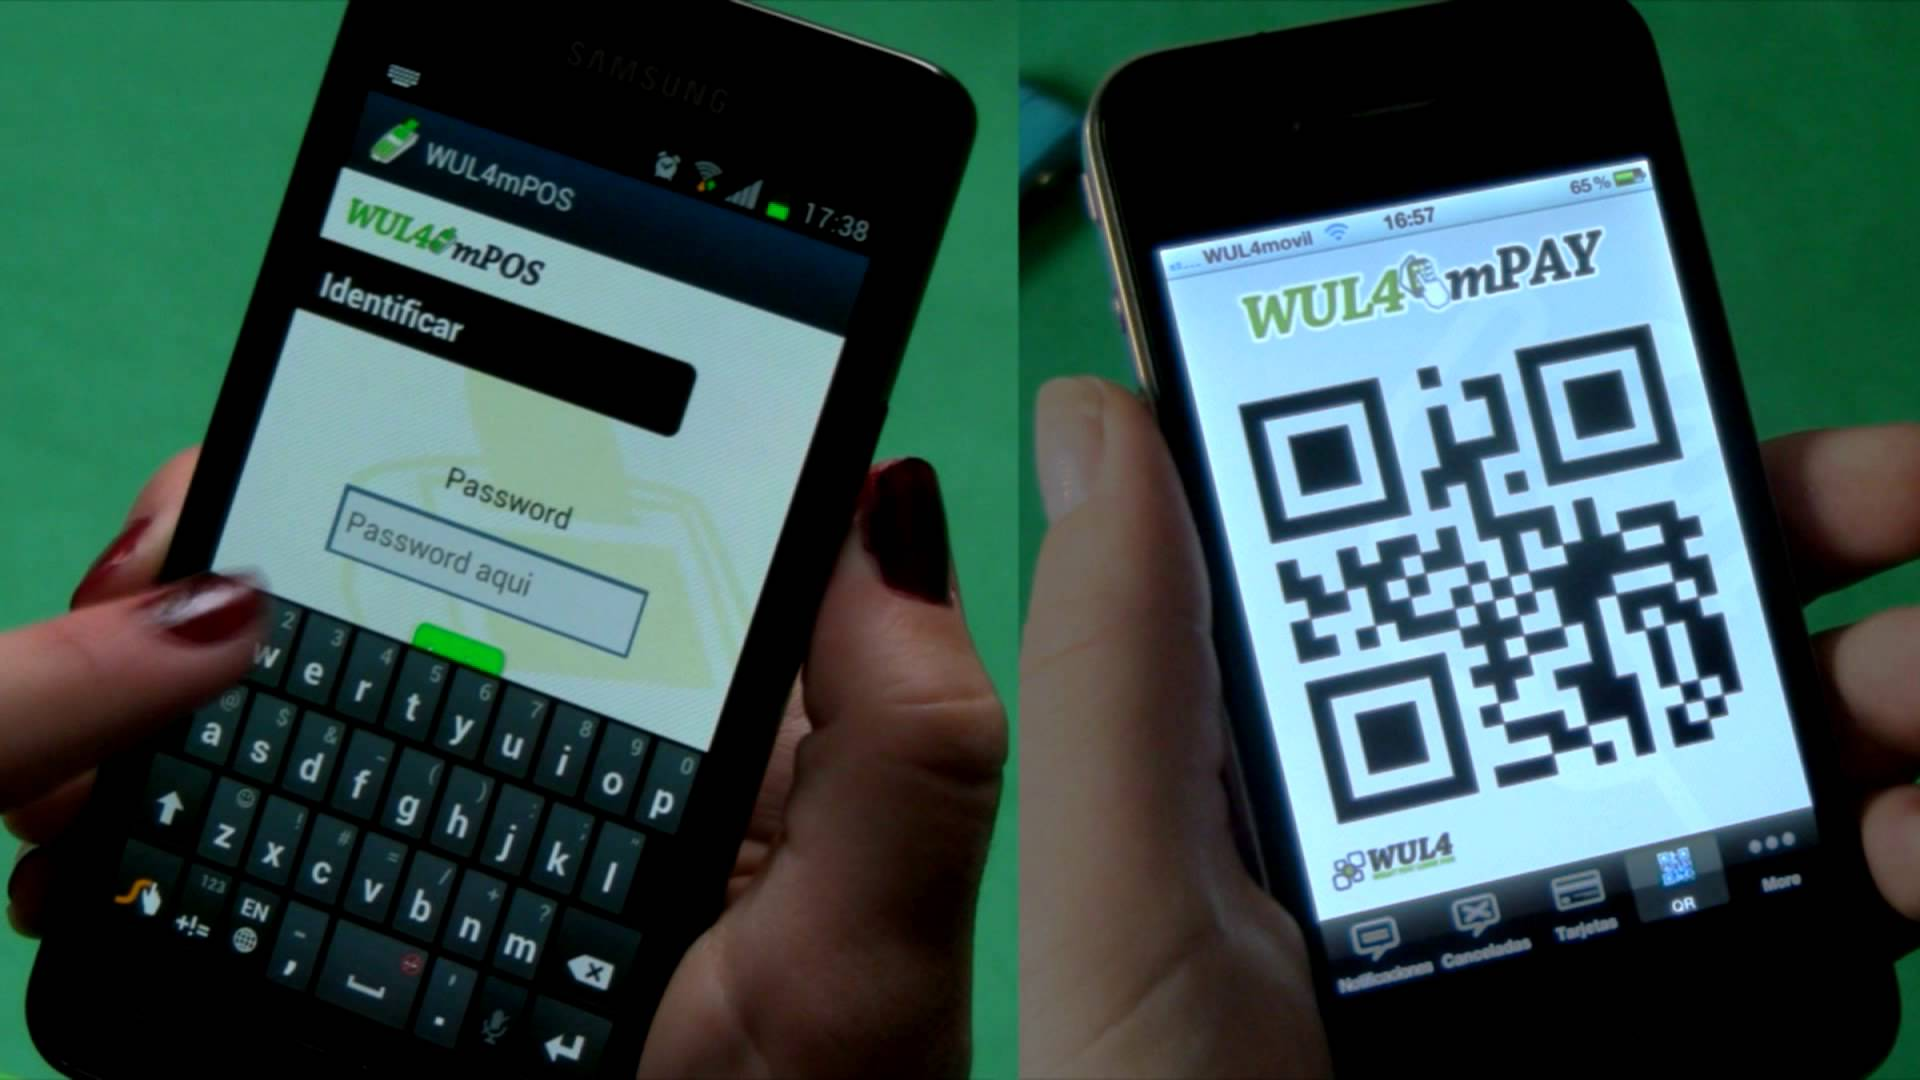
\includegraphics[height=1in]{imgs/wul4mpay.jpg}}}$
  $\vcenter{\hbox{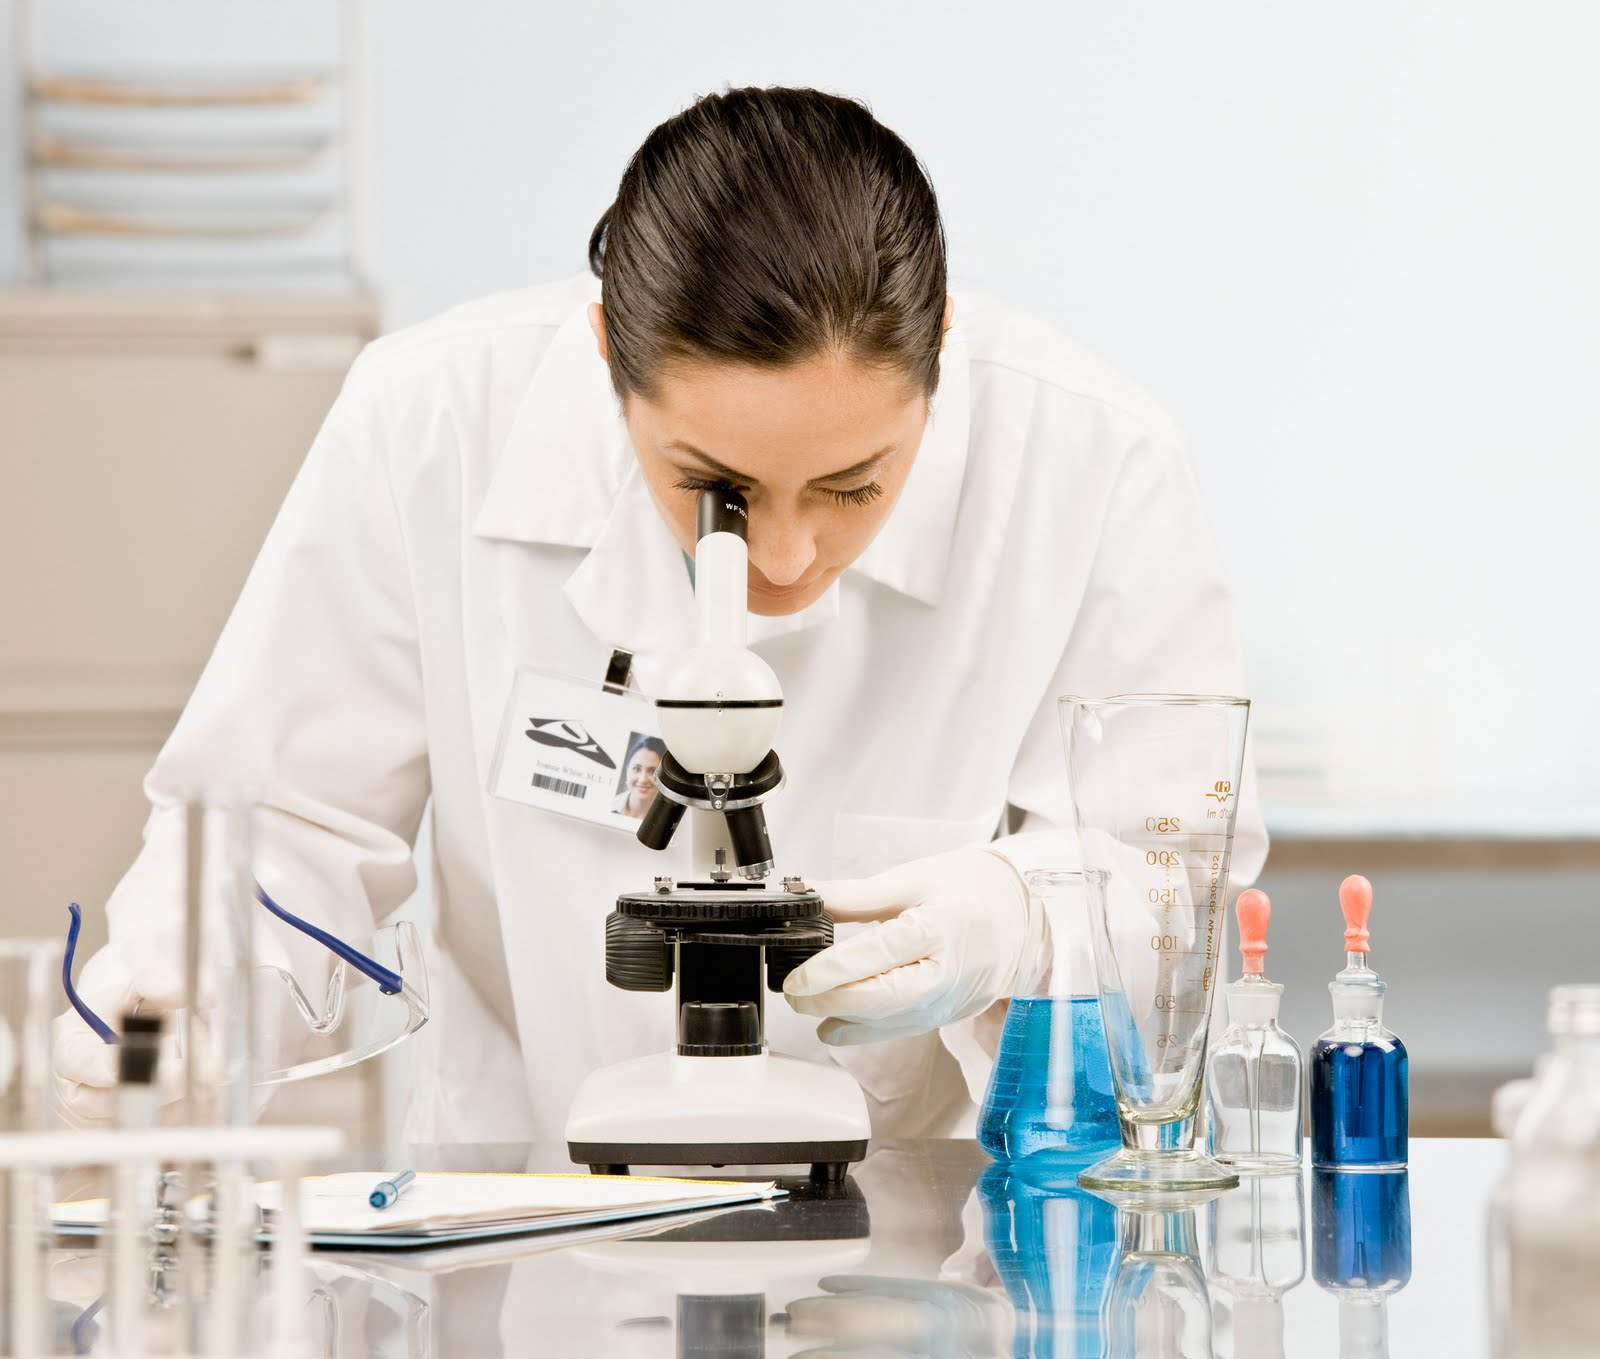
\includegraphics[height=1in]{imgs/id.jpg}}}$
\end{itemize}
}

\section{¿Realidad aumentada?}
\frame
{
\frametitle{Definición de realidad aumentada}
\begin{itemize}
  \item Superposición de \textbf{información virtual} sobre entornos reales a partir de una aplicación informática
  \item ¿Qué necesitamos?

  \begin{itemize}
    \item Una \textbf{pantalla} donde poder ver esta información añadida 
    \item Un software que, controlando una \textbf{cámara}, un \textbf{sensor} o un \textbf{GPS} e interpretando los patrones o coordenadas del mundo real, nos generará esta \textbf{información}
  \end{itemize}

  \item Multitud de aplicaciones
\end{itemize}
}
\section{Aplicaciones}
\frame
{
\frametitle{Aplicaciones de realidad aumentada}
{\setlength{\arrayrulewidth}{0mm}
  \begin{tabular}{| c | c |}
  \hline
  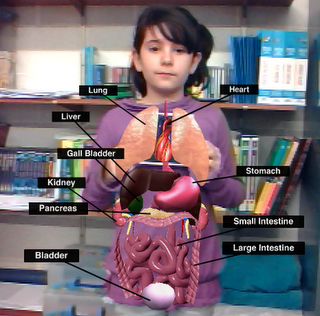
\includegraphics[height=4cm]{imgs/raeducacion.png} & 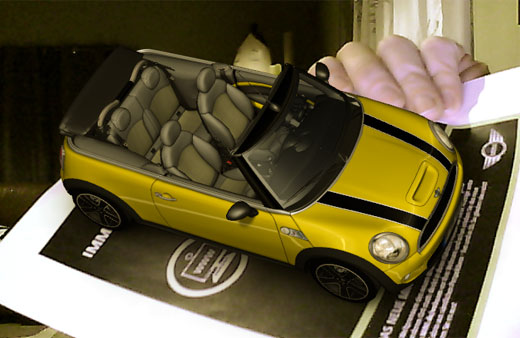
\includegraphics[height=4cm]{imgs/minira.jpg}\\
  \hline
  Educación & Marketing / Publicidad\\
  \hline
  \end{tabular}
}
}

\frame
{
\frametitle{Aplicaciones de realidad aumentada}
{\setlength{\arrayrulewidth}{0mm}
  \begin{tabular}{| c | c |}
  \hline
  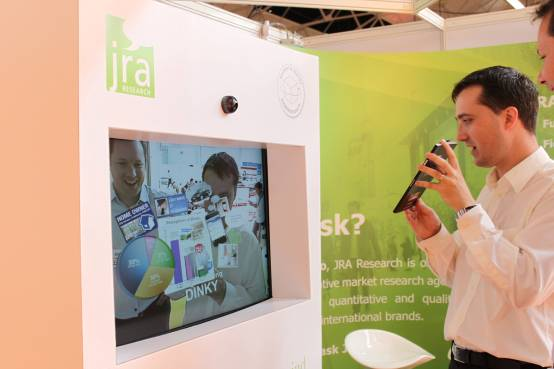
\includegraphics[height=3.5cm]{imgs/event-ra.jpg} & 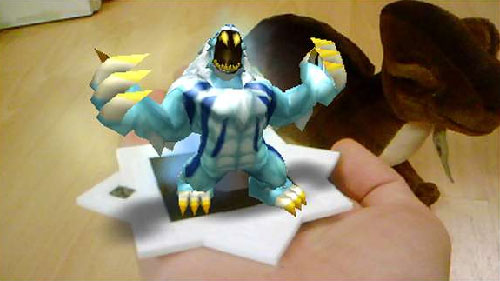
\includegraphics[height=3.5cm]{imgs/invizimals.jpg}\\
  \hline
  Eventos & Videojuegos\\
  \hline
  \end{tabular}
}
}

\section{RA en Android}
\frame
{
\frametitle{¿Qué opciones hay?}
{\setlength{\arrayrulewidth}{0mm}
\begin{table}[ht]
  \centering
  \begin{tabular}{| m{3cm} | m{4cm} | m{4cm} |}
  \hline
  
\includegraphics[height=2cm, width=1.8cm]{imgs/opencv.png} & 
     \hspace{2cm}
\includegraphics[width=3cm]{imgs/vuforia.png} & 
     \hspace{2cm}
\includegraphics[width=3cm]{imgs/metaio.jpg}
  \end{tabular}
\end{table}
}

{\setlength{\arrayrulewidth}{0mm}
\begin{table}[ht]
  \centering
  \begin{tabular}{| m{4cm} | m{4cm} |}
  \hline
  
\includegraphics[width=2cm]{imgs/layar.jpg}& 
\includegraphics[width=2cm]{imgs/wikitude.png}
  \end{tabular}
\end{table}
}
}

\subsection*{OpenCV}
\frame
{
\frametitle{OpenCV for Android}
\begin{itemize}
 \item Biblioteca libre de \textbf{visión artificial} originalmente desarrollada por \textbf{Intel}
 \item En 2008, la empresa \textbf{Willow Garage} asume el soporte. En 2012, lo hace la empresa \textbf{ItSeez}.
 \item Disponible para Windows, Linux, Mac, Android e iOS
 \item Para Android se proporciona la API Java con clases específicas, que es un subconjunto de la API de C
 \item SDK Quick start\\ \url{http://docs.opencv.org/doc/tutorials/introduction/android_binary_package/O4A_SDK.html}
 \item Utilizado en aeronaves no tripuladas, sistemas de vigilancia, reconocimiento facial, etc.
\end{itemize}
}

\frame
{
\frametitle{OpenCV for Android: ventajas e inconvenientes}
\begin{itemize}
\item \textbf{Ventajas:}
  \begin{itemize}
   \item Licencia BSD
   \item Buen rendimiento
   \item Multiplataforma
   \item Soporte de la comunidad. Multitud de snippets.
  \end{itemize}

\item \textbf{Inconvenientes:}
  \begin{itemize}
   \item La API de Java es un subconjunto mínimo. Para obtener un conjunto mayor, se recomienda usar el NDK + JNI. Más info: \\
     \url{http://www.nacho-alvarez.es/index.php/blog/2012/05/02/conectar-programas-cc-con-aplicaciones-android/}
   \item El sobreimpresionado de elementos debe hacerse manualmente
   \item Se centra en visión por computador, así que no tenemos la parte GPS
   \item Hace falta una formación específica en visión artificial para utilizarla correctamente
  \end{itemize}

\end{itemize}
}

\frame
{
\frametitle{OpenCV for Android: recursos}
\begin{itemize}
\item \textbf{OpenCV4Android:} \url{http://opencv.org/platforms/android.html}
\item \textbf{Quick Start:} \url{http://docs.opencv.org/doc/tutorials/introduction/android_binary_package/O4A_SDK.html}
\item \textbf{Android development with OpenCV:} \url{http://docs.opencv.org/doc/tutorials/introduction/android_binary_package/dev_with_OCV_on_Android.html}
\item \textbf{Java API:} \url{http://docs.opencv.org/java/}
\end{itemize}
}

\subsection*{Vuforia}
\frame
{
\frametitle{Vuforia}
\begin{itemize}
 \item Biblioteca que permite reconocer y hacer el seguimiento de imágenes planas (Image Targets) y objetos 3D simples
 \item Desarrollo de Qualcomm Austria Research Center Gmbh
 \item Disponible para Android, iOS y Unity
 \item Incluye la parte NDK + JNI pre-compilada. Sólo tenemos que incluir las bibliotecas y llamar a los métodos nativos.
 \item Targets disponibles: Image, Cylinder, Text-Word, User-defined, Cloud Recognition, Multi-Targets, Frame markers y Virtual buttons.
\end{itemize}
}

\frame
{
\frametitle{Vuforia: Cloud Recognition}
 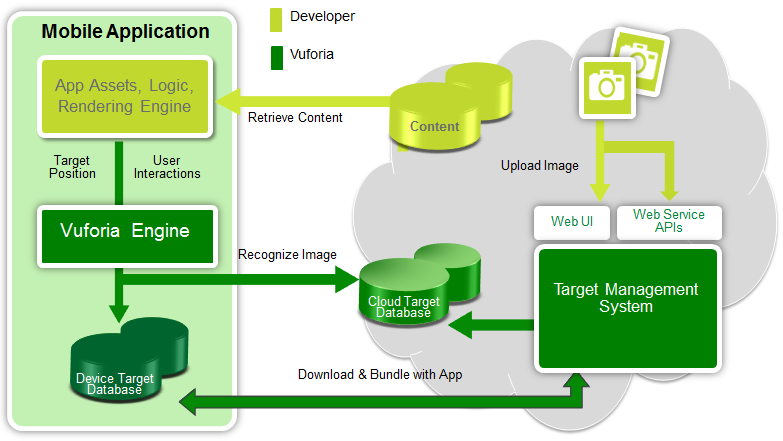
\includegraphics[width=12cm]{imgs/vuforia-components.png}
}

\frame
{
\frametitle{Vuforia: ventajas e inconvenientes}
\begin{itemize}
\item \textbf{Ventajas:}
  \begin{itemize}
   \item Licencia QTL: gratuito y puede usarse en apps comerciales
   \item Gran rendimiento
   \item Posibilidad de reconocimiento en la nube
   \item Clases más sencillas que en OpenCV
  \end{itemize}

\item \textbf{Inconvenientes:}
  \begin{itemize}
   \item Dependencia de NDK + JNI. Si se quiere ampliar, se amplían los métodos nativos.
   \item Cloud recognition no es totalmente gratuito y no podemos montar nuestro propio server
   \item Se centra en visión por computador, así que no tenemos la parte GPS
   \item Foro de debate, con menor orientación a comunidad
  \end{itemize}

\end{itemize}
}

\frame
{
\frametitle{Vuforia: recursos}
\begin{itemize}
\item \textbf{Descarga SDK:} \url{https://developer.vuforia.com/resources/sdk/android}
\item \textbf{Instalación SDK:} \\\url{https://developer.vuforia.com/resources/dev-guide/step-2-installing-vuforia-sdk}
\item \textbf{Target Manager:} \url{https://developer.vuforia.com/targetmanager/project/checkDeviceProjectsCreated?dataRequestedForUserId=}
\item \textbf{Sample apps:} \url{https://developer.vuforia.com/resources/sample-apps}
\end{itemize}
}

\subsection*{Metaio}
\frame
{
\frametitle{Metaio}
\begin{itemize}
 \item Fundado en 2003 en Munich por Thomas Alt y Peter Meier
 \item Se estructura en \textit{canales}
 \item Ofrecen un conjunto de productos:
 \begin{itemize}
   \item \textbf{metaio SDK + metaio Cloud:} SDK de desarrollo para metaio con cuenta de acceso a Cloud. 
   \item \textbf{metaio Creator + metaio Cloud:} aplicación de escritorio para crear AR channels y visualizarlo en junaio.
   \item \textbf{junaio:} navegador de realidad aumentada.
 \end{itemize}
 \item Disponible para Android, iOS y Windows
\end{itemize}
}

\frame
{
\frametitle{Junaio: ventajas e inconvenientes}
\begin{itemize}
\item \textbf{Ventajas:}
  \begin{itemize}
   \item Posibilidad de reconocimiento en la nube
   \item Posibilidad de montar tu propia nube
   \item SDK muy sencillo y bien documentado
   \item Buen soporte orientado a comunidad de desarrolladores
  \end{itemize}

\item \textbf{Inconvenientes:}
  \begin{itemize}
   \item Pequeño lag a veces
   \item Eliminar la marca de agua es caro
   \item No es libre
   \item La plataforma web es demasiado compleja 
  \end{itemize}

\end{itemize}
}

\subsection*{Layar}
\frame
{
\frametitle{Layar}
\begin{itemize}
 \item Fundado en 2009 en Amsterdam por Raimo van der Klein, Claire Boonstra y Maarten Lens-FitzGerald
 \item Se estructura en \textit{campañas}
 \item También proporciona acceso a su propia nube privada\\
   \url{https://www.layar.com/creator/}
 \item Disponible para Android e iOS
 \item Utilizado por Nissan, Ford, Philips, WWF Panda, Dan Brown...
\end{itemize}
}

\frame
{
\frametitle{Layar: ventajas e inconvenientes}
\begin{itemize}
\item \textbf{Ventajas:}
  \begin{itemize}
   \item Reconocimiento de imágenes por encima de la media
   \item Posibilidad de reconocimiento en la nube
   \item Web perfectamente preparada para la creación de campañas
  \end{itemize}

\item \textbf{Inconvenientes:}
  \begin{itemize}
   \item Pobre soporte y documentación
   \item Eliminar la marca de agua es más caro incluso que Metaio (7000\euro/año)
   \item No es libre
   \item No permite montar un servidor de recursos propios
  \end{itemize}

\end{itemize}
}

\frame
{
\frametitle{Layar: recursos}
\begin{itemize}
\item \textbf{Descarga SDK:} \\\url{https://www.layar.com/products/custom-solutions/sdk/request/}
\item \textbf{Target Manager:} \\\url{https://www.layar.com/creator/}
\item \textbf{Foro de desarrolladores:} \\\url{http://devsupport.layar.com/home}
\item \textbf{Planes de precios:} \\\url{https://www.layar.com/pricing/}
\end{itemize}
}

\subsection*{Wikitude}
\frame
{
\frametitle{Wikitude}
\begin{itemize}
 \item Lanzamiento inicial en 2008 en Austria por la empresa Wikitude Gmbh
 \item Se estructura en \textit{worlds}
 \item También proporciona acceso a su propia nube privada\\
   \url{http://studio.wikitude.com}
 \item Disponible para Android, iOS, BlackBerry, Windows Phone, Phonegap y Titanium
 \item Ganador del premio \textit{Best Augmented Reality Browser, Augmented Planet} en 2009, 2010, 2011 y 2012, entre muchos otros
\end{itemize}
}

\frame
{
\frametitle{Wikitude: ventajas e inconvenientes}
\begin{itemize}
\item \textbf{Ventajas:}
  \begin{itemize}
   \item Documentación muy completa
   \item Más barato que Metaio y Layar (600\euro), incluyendo geolocalización
   \item Versión educacional con marca de agua a 0\euro
   \item Posibilidad de reconocimiento en la nube
   \item Web perfectamente preparada para la creación de campañas
   \item Soporte muy orientado a comunidad
  \end{itemize}

\item \textbf{Inconvenientes:}
  \begin{itemize}
   \item No es libre
   \item No permite montar un servidor de recursos propios
  \end{itemize}

\end{itemize}
}

\frame
{
\frametitle{Wikitude: recursos}
\begin{itemize}
\item \textbf{Descarga SDK:} \url{http://developer.wikitude.com/download}
\item \textbf{Construir worlds con Google Maps:} \\\url{http://www.wikitude.com/build-wikitude-world-google-collaborative-maps/}
\item \textbf{Publicar world:} \\\url{http://devzone.wikitude.com/web/forum/tools/publish-in-wikitude}
\item \textbf{Target Manager:} \url{http://developer.wikitude.com/tools/target-manager/?level=0}
\item \textbf{Foro de desarrolladores:} \url{http://developer.wikitude.com/developer-forum}
\item \textbf{Ejemplos Android:} \url{http://developer.wikitude.com/documentation/android}
\end{itemize}
}

\section{Demo}
\frame
{
\frametitle{Vídeos}
{
\begin{itemize}
  \item \textbf{IR simple matching}: \textit{Wikitude Examples -> 1. Image Recognition -> 1.1. Image On Target ->} \url{http://youtu.be/wbz0N7TQRCA}
  \item \textbf{IR multiple targets}: \textit{Wikitude Examples -> 1. Image Recognition -> 1.2. Multiple Targets ->} \url{http://youtu.be/lIA3YItmO80}
  \item \textbf{IR con playback de video}: \textit{Wikitude Examples -> 6. Video -> 6.2. Playback States ->} \url{http://youtu.be/XZCaRuSka_k}
  \item \textbf{IR mostrando vídeo transparente}: \textit{Wikitude Examples -> 6. Video -> 6.4. Bonus-Transparent Video ->} \url{http://youtu.be/VfavE33ZSnk}
  \item \textbf{Gestión de POIs en geolocalización}: \textit{Wikitude Examples -> 5. Browsing POIs -> 5.5. Native Detail Screen ->} \url{http://youtu.be/OEyqvsoExDA}
  \item \textbf{Integración en aplicación propia}: \textit{My own app ->} \url{http://youtu.be/nscPzcGQfQ8}
\end{itemize}
}
}

\frame
{
\frametitle{Demostración}
{
\begin{table}[ht]
  \centering
  \begin{tabular}{c}
    
\includegraphics[height=7.5cm]{imgs/demo.jpg}
  \end{tabular}
\end{table}
}
}

\section{Conclusiones}
\frame
{
\frametitle{Conclusiones personales}
\begin{itemize}
 \item Vuforia es ideal como herramienta libre para desarrollar una aplicación de realidad aumentada con reconocimiento de imágenes
 \item Sin embargo, la parte de geolocalización habría que desarrollarla manualmente
 \item Para pequeñas aplicaciones, podemos utilizar Wikitude que tiene una versión Edu gratuita con marca de agua
 \item Igualmente, para aplicaciones comerciales de peso, la inversión de Wikitude es de 600\euro \hspace{0.15cm}en un único pago y de 9\euro/mes por el uso de 3 imágenes en su nube
\end{itemize}
}


\end{document}